\chapter{Practical Implementation and Experimental Results}
\label{chap:ch3_practical}

\par This chapter forms the core practical component of the thesis, delineating the end-to-end engineering lifecycle of the AI-assisted dental imaging platform. It transitions the theoretical paradigms established in previous chapters into a concrete, functioning software architecture. The discourse is systematically organized to address the foundational problem, the methodological research design, the intricate system architecture, the explicit implementation nuances of the machine learning pipeline, and finally, a rigorous empirical evaluation of the resultant model.

\section{Problem Definition and Approach}
\label{sec:ch4_problem_approach}

\subsection{Concrete Description of the Problem}
\par The diagnostic interpretation of panoramic and bitewing dental radiographs remains a highly subjective and cognitively demanding task within modern endodontics and restorative dentistry. Clinical practitioners are routinely confronted with the challenge of detecting microscopic pathological manifestations—such as incipient enamel caries or early-stage periapical radiolucencies—against a background of highly overlapping anatomical structures, varying exposure contrasts, and visual artifacts induced by pre-existing metallic restorations. This inherent diagnostic ambiguity frequently culminates in observational fatigue, directly escalating the rate of false-negative diagnoses wherein critical early interventions are missed.
\par Furthermore, the application of generalized computer vision models to this specific domain has historically proven inadequate. Conventional single-stage object detectors frequently fail to isolate densely clustered anomalies (e.g., multiple proximal caries on adjacent teeth) due to aggressive spatial down-sampling and overlapping bounding box conflicts. 

\subsection{Delineation and Presentation of the Developed Solution}
\par To mitigate these profound clinical and technical deficiencies, this research engineered a dedicated, web-based diagnostic support ecosystem powered by a meticulously fine-tuned Faster R-CNN object detection architecture. The proposed solution operates as an asynchronous, highly secure client-server application. 
\par The foundational approach dictates that raw radiographic uploads are intercepted by a Python-based FastAPI backend, which immediately routes the tensor data to the trained PyTorch inference engine. Rather than relying on generic resolution scaling, the model was explicitly constrained to evaluate inputs at extreme high resolutions to preserve granular pixel densities. Subsequent to the tensorial evaluation, a secondary algorithmic filtering mechanism natively suppresses redundant spatial overlaps, ensuring that the clinical user interface displays only mathematically validated, distinct pathological entities. This approach guarantees an optimal balance between maximal diagnostic sensitivity and strict specificity, significantly outperforming rudimentary single-stage counterparts in resolving densely grouped dental anomalies.

\section{Methodology and Research Design}
\label{sec:ch4_methodology}

\subsection{Research Design and Data Engineering}
\par The methodological framework of this thesis follows an iterative, experimental applied-research paradigm. The primary objective was to construct a statistically robust training pipeline capable of generalizing across varied clinical environments.
\par The research design necessitated profound dataset engineering. The foundational data utilized in this research is derived from the \textbf{DENTEX dataset} (originally associated with the Dentex Challenge), which provides a comprehensive benchmark for dental object detection. The dataset consisted of 705 rigorously annotated panoramic radiographs, distributed across discrete diagnostic classes. A pivotal methodological decision involved the dynamic re-mapping of ontological categories to optimize neural network convergence. Initial evaluations indicated that delineating "Deep Caries" from standard "Caries" introduced severe class imbalance and gradient instability, as the morphological boundaries between the two are radiographically ambiguous. Consequently, the taxonomy was algorithmically unified during early training iterations. However, subsequent methodological refinements successfully re-isolated "Deep Caries" as an independent diagnostic entity to maximize the granularity of the clinical output, mapping it alongside distinct classifications for "Periapical Lesions" and "Impacted Teeth."

\subsection{Applied Methods and Data Augmentation}
\par To combat the risk of over-fitting and to ensure the network generalizes effectively to unseen clinical data, targeted geometric data augmentation methodologies were applied during the stochastic training phases. The PyTorch \texttt{torchvision.transforms.v2} library was utilized to construct a dynamic preprocessing pipeline. The transformations included \texttt{RandomHorizontalFlip(p=0.5)} and \texttt{RandomAffine} operations with a 5-degree rotational variance, alongside translation (\(\pm 3\%\)) and scaling bounds (0.95 to 1.05). Furthermore, a critical \texttt{SanitizeBoundingBoxes} transformation with a \texttt{min\_size} threshold of 1.0 pixel was enforced to computationally discard invalid or degraded coordinate artifacts post-augmentation. These combined spatial augmentations forced the convolutional backbone to learn the absolute geometric morphology of the caries and lesions rather than memorizing their exact spatial orientation within the training subset.

\begin{figure}[htbp]
    \centering
    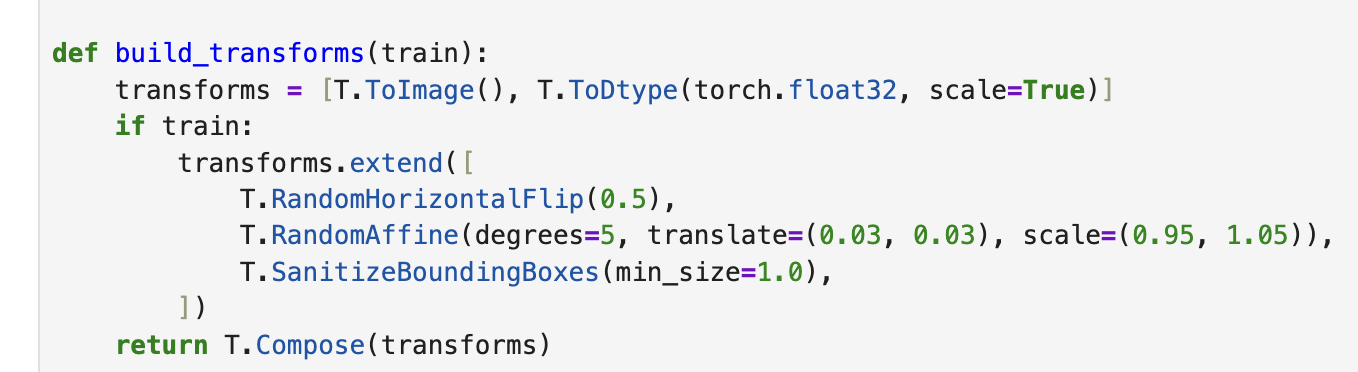
\includegraphics[width=1.0\textwidth]{figures/augmentations.png}
    \caption{Visual representation of the data augmentation pipeline applied during the training phase, highlighting the geometric affine transformations and horizontal flipping.}
    \label{fig:augmentations}
\end{figure}

\section{System Overview and Architecture}
\label{sec:ch4_architecture}

\subsection{Overall Structural Paradigm}
\par The developed solution is architected upon a decoupled, microservice-inspired Client-Server paradigm, ensuring absolute modularity and independent scalability of the machine learning inference engine.
\par The architecture is broadly partitioned into three interconnected strata: the frontend presentation layer, the backend orchestration layer, and the deep learning inference core. This deliberate decoupling guarantees that the extreme computational load of the tensorial matrix multiplications does not disrupt the asynchronous flow of HTTP requests originating from the clinician's web dashboard.

\subsection{Component Description and Data Flow}
\par The operational data flow is initiated within the React.js frontend interface. A practitioner uploads a target radiograph, which is encoded and securely transmitted via an HTTP POST request to the FastAPI backend framework.
\par \textbf{FastAPI Orchestrator:} Upon receiving the payload, the FastAPI controller immediately decodes the binary image stream into a format viable for mathematical processing. It instantiates the pre-loaded PyTorch model state dictionary (\texttt{best6mai.pth}), completely avoiding the massive latency overhead of reloading the model weights into memory for sequential requests.
\par \textbf{PyTorch Inference Core:} The decoded image matrix is normalized and transformed into a multidimensional tensor. The Faster R-CNN architecture processes this tensor through its ResNet-50 backbone, generating region proposals and subsequently executing the final classification and bounding box regression operations. 

\begin{figure}[htbp]
    \centering
    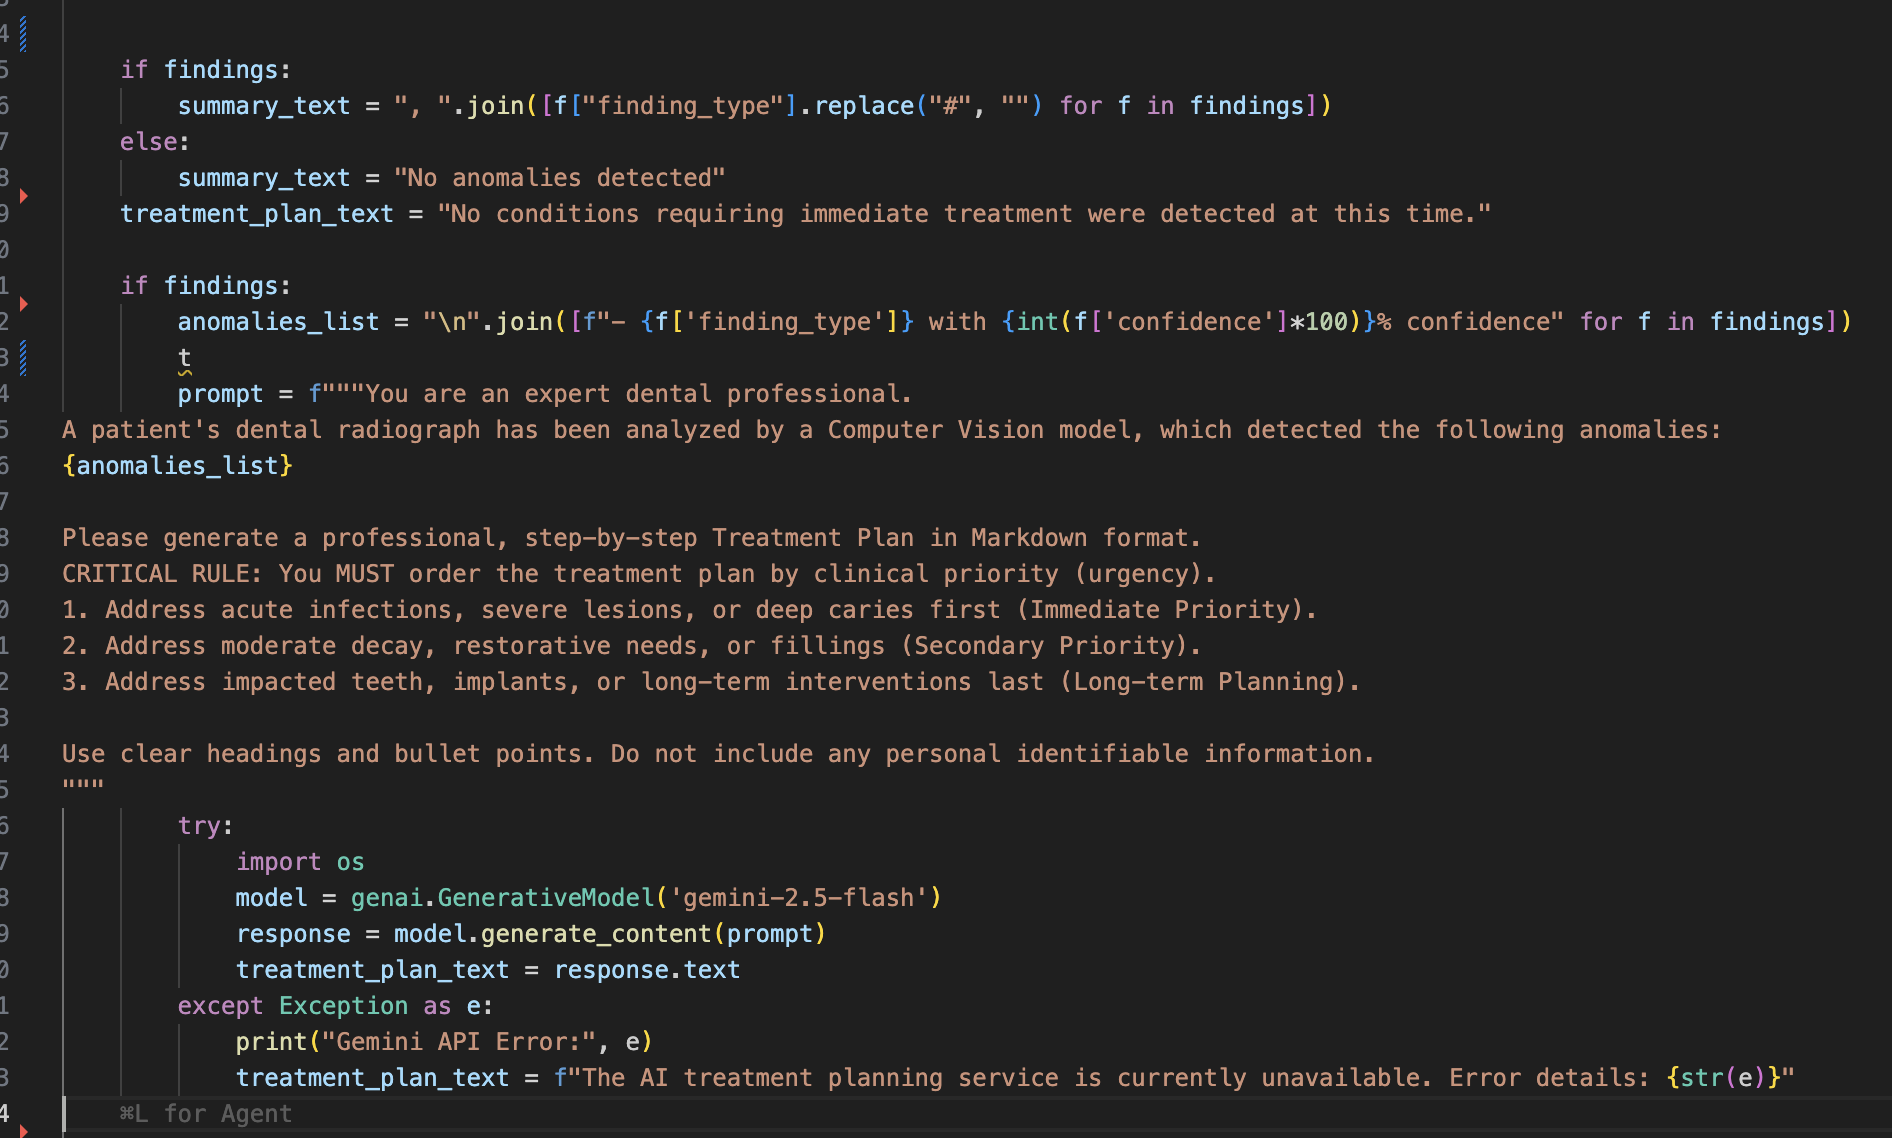
\includegraphics[width=0.9\textwidth]{figures/prompt.png}
    \caption{The structured clinical prompt designed for the LLM integration, illustrating the prioritization logic and diagnostic context passed to the model.}
    \label{fig:ai_prompt}
\end{figure}

\par \textbf{Post-Processing and Treatment Planning:} The raw tensor outputs are intercepted by a custom post-processing script. After applying Non-Maximum Suppression to eliminate intersecting coordinate geometries, the backend constructs a structured JSON payload detailing the classified pathologies, their coordinates, and confidence metrics. Crucially, the system extends beyond simple detection by incorporating an \textbf{automated treatment planning} module. By utilizing the diagnostic metadata as a structured \textbf{contextual prompt} for an integrated Large Language Model, the backend generates personalized clinical recommendations for each detected anomaly. The React frontend intercepts this enriched JSON response, rendering color-coded SVG overlays while simultaneously presenting the clinician with a comprehensive, AI-generated therapeutic roadmap.



\subsection{Clinical Workflow and Data Persistence}
\par The platform is engineered as a multi-user clinical environment, where each practitioner maintains a private, authenticated workspace. Upon successful authentication, doctors gain access to a personalized dashboard containing their unique patient registry.

\begin{figure}[htbp]
    \centering
    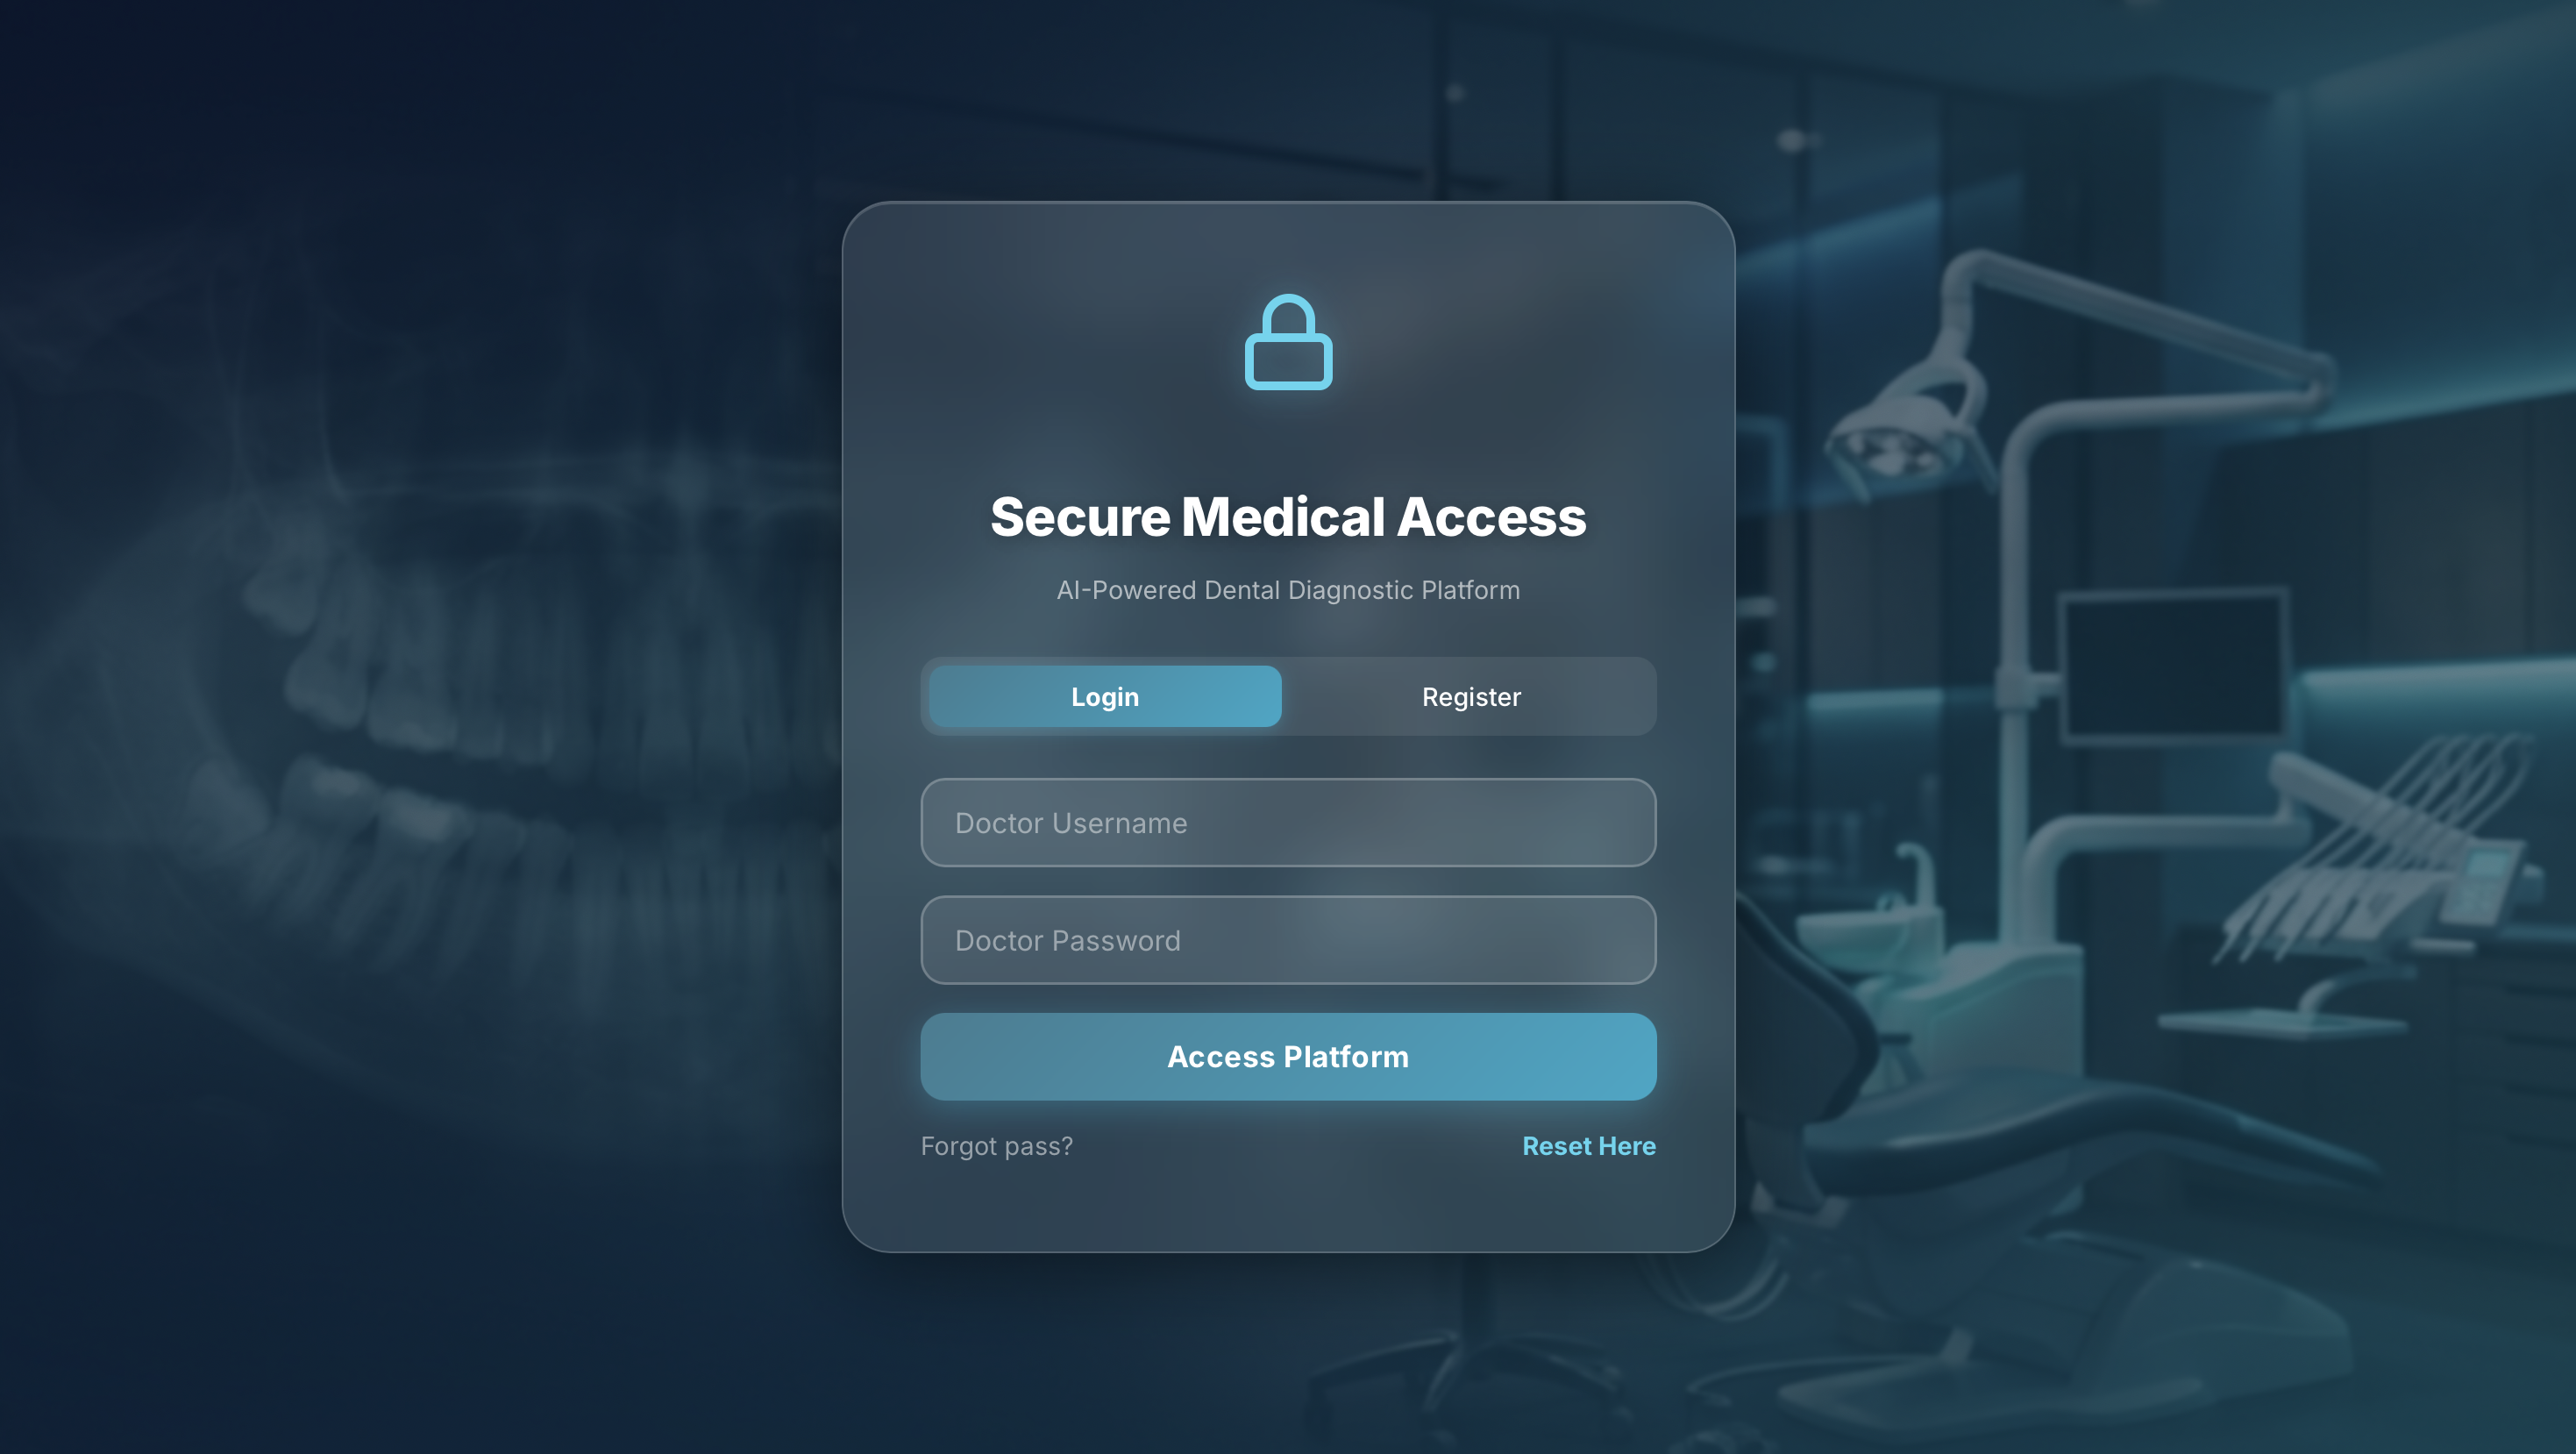
\includegraphics[width=0.8\textwidth]{figures/medical_acces.png}
    \caption{The clinician authentication interface, providing a secure entry point to the personalized dental diagnostic workspace.}
    \label{fig:login_screen}
\end{figure}
\par \textbf{Patient Data Management:} The diagnostic workflow begins with the registration of patient metadata, including the patient's full name and age. This structured data is persisted within a relational database, establishing a robust link between the clinical history and the radiographic findings. Following the diagnostic evaluation, the system provides a comprehensive export utility, allowing practitioners to download a unified report containing the localized radiographic findings and the AI-generated treatment plan for offline clinical record-keeping.
\par \textbf{Analytical Dashboard:} To facilitate long-term clinical monitoring, the system integrates a dynamic \textbf{analytics chart}. This visualization layer aggregates diagnostic trends across the doctor's entire patient base, providing a high-level statistical overview of localized pathologies (e.g., the prevalence of caries vs. impacted teeth). This data-driven dashboard empowers clinicians to identify recurring patterns within their patient population and optimize their overall diagnostic accuracy.


\section{Implementation and Technical Execution}
\label{sec:ch4_implementation}

\subsection{Technologies and Frameworks}
\par The implementation phase was strictly dictated by industry-standard deep learning and web engineering frameworks. The neural network architecture was engineered utilizing \textbf{PyTorch} and its dedicated \textbf{Torchvision} library, exploiting their unparalleled support for dynamic computational graphs and robust tensor manipulation. The backend infrastructure was constructed using \textbf{FastAPI}, chosen explicitly for its native ASGI (Asynchronous Server Gateway Interface) concurrency, which allows non-blocking execution of deep learning models. The client interface was developed in \textbf{React.js}, leveraging its virtual DOM to instantly render complex geometric bounding boxes without page reload interruptions.

\subsection{Key Algorithms and Architectural Decisions}
\par Several critical algorithmic decisions were implemented to bridge the gap between theoretical computer vision and functional clinical utility.

\par \textbf{Resolution Scaling During Inference:}
Standard pre-trained object detectors enforce aggressive image down-sampling (typically capping the minimal axis at 800 pixels) to accelerate inference speeds. Given that dental radiographs often exceed 2500 pixels in width, this default behavior catastrophically "crushed" the pixel density of incipient caries during the diagnostic prediction phase. While the standard resolution was maintained during the resource-intensive training phase to allow for a viable batch size, the inference engine constructor within the backend was explicitly overridden to process extreme resolutions:
\begin{figure}[htbp]
    \centering
    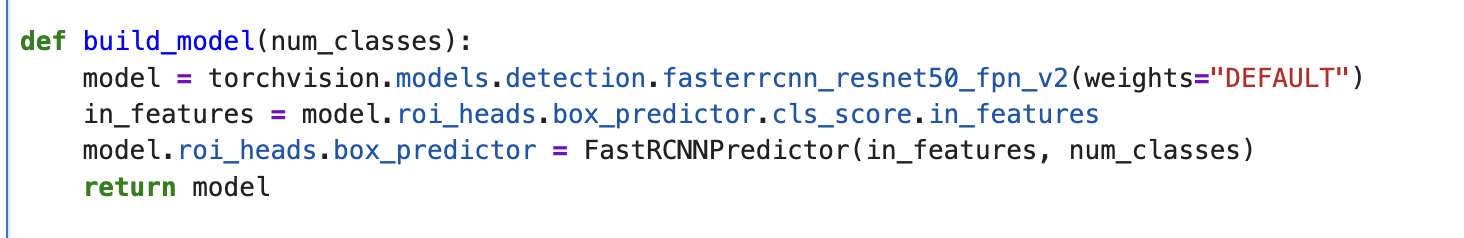
\includegraphics[width=0.8\textwidth]{figures/build_model.png}
    \caption{The implementation of the \texttt{build\_model} function, demonstrating the initialization of the Faster R-CNN architecture with pre-trained ResNet-50 weights and the customized classification head.}
    \label{fig:build_model_code}
\end{figure}
This critical design decision during deployment forces the architecture to process nearly double the standard pixel volume, retaining the high-frequency structural details crucial for the backend to accurately identify micro-lesions.

\par \textbf{Batched Non-Maximum Suppression (NMS):}
A pervasive issue in evaluating densely packed dental anomalies is the generation of redundant bounding boxes over the same tooth. Initial manual geometric intersection algorithms proved inadequate, occasionally leaving overlapping artifacts. To permanently resolve this, the native PyTorch \texttt{batched\_nms} algorithm was integrated directly into the inference loop.
\begin{verbatim}
keep_indices = torchvision.ops.batched_nms(
    boxes, scores, labels, iou_threshold=0.15
)
\end{verbatim}
By enforcing an extremely aggressive Intersection over Union (IoU) threshold of 0.15, the system guarantees that any bounding boxes of the same class overlapping by more than 15\% are mathematically fused, retaining only the prediction with the highest confidence score. This results in an exceptionally clean, clinically legible visual output.

\par \textbf{Optimization Algorithm:}
To ensure stable and efficient backpropagation across the deep convolutional layers, the \texttt{AdamW} (Adam with Weight Decay) optimizer was selected. Configured with a conservative learning rate of \(1e^{-4}\), the optimizer effectively mitigates the risk of aggressive weight updates that could destabilize the Region Proposal Network. The decoupled weight decay mechanism native to AdamW provides superior regularization, preventing the model from over-fitting to the specific training dataset during its extended training cycle.

\begin{figure}[htbp]
    \centering
    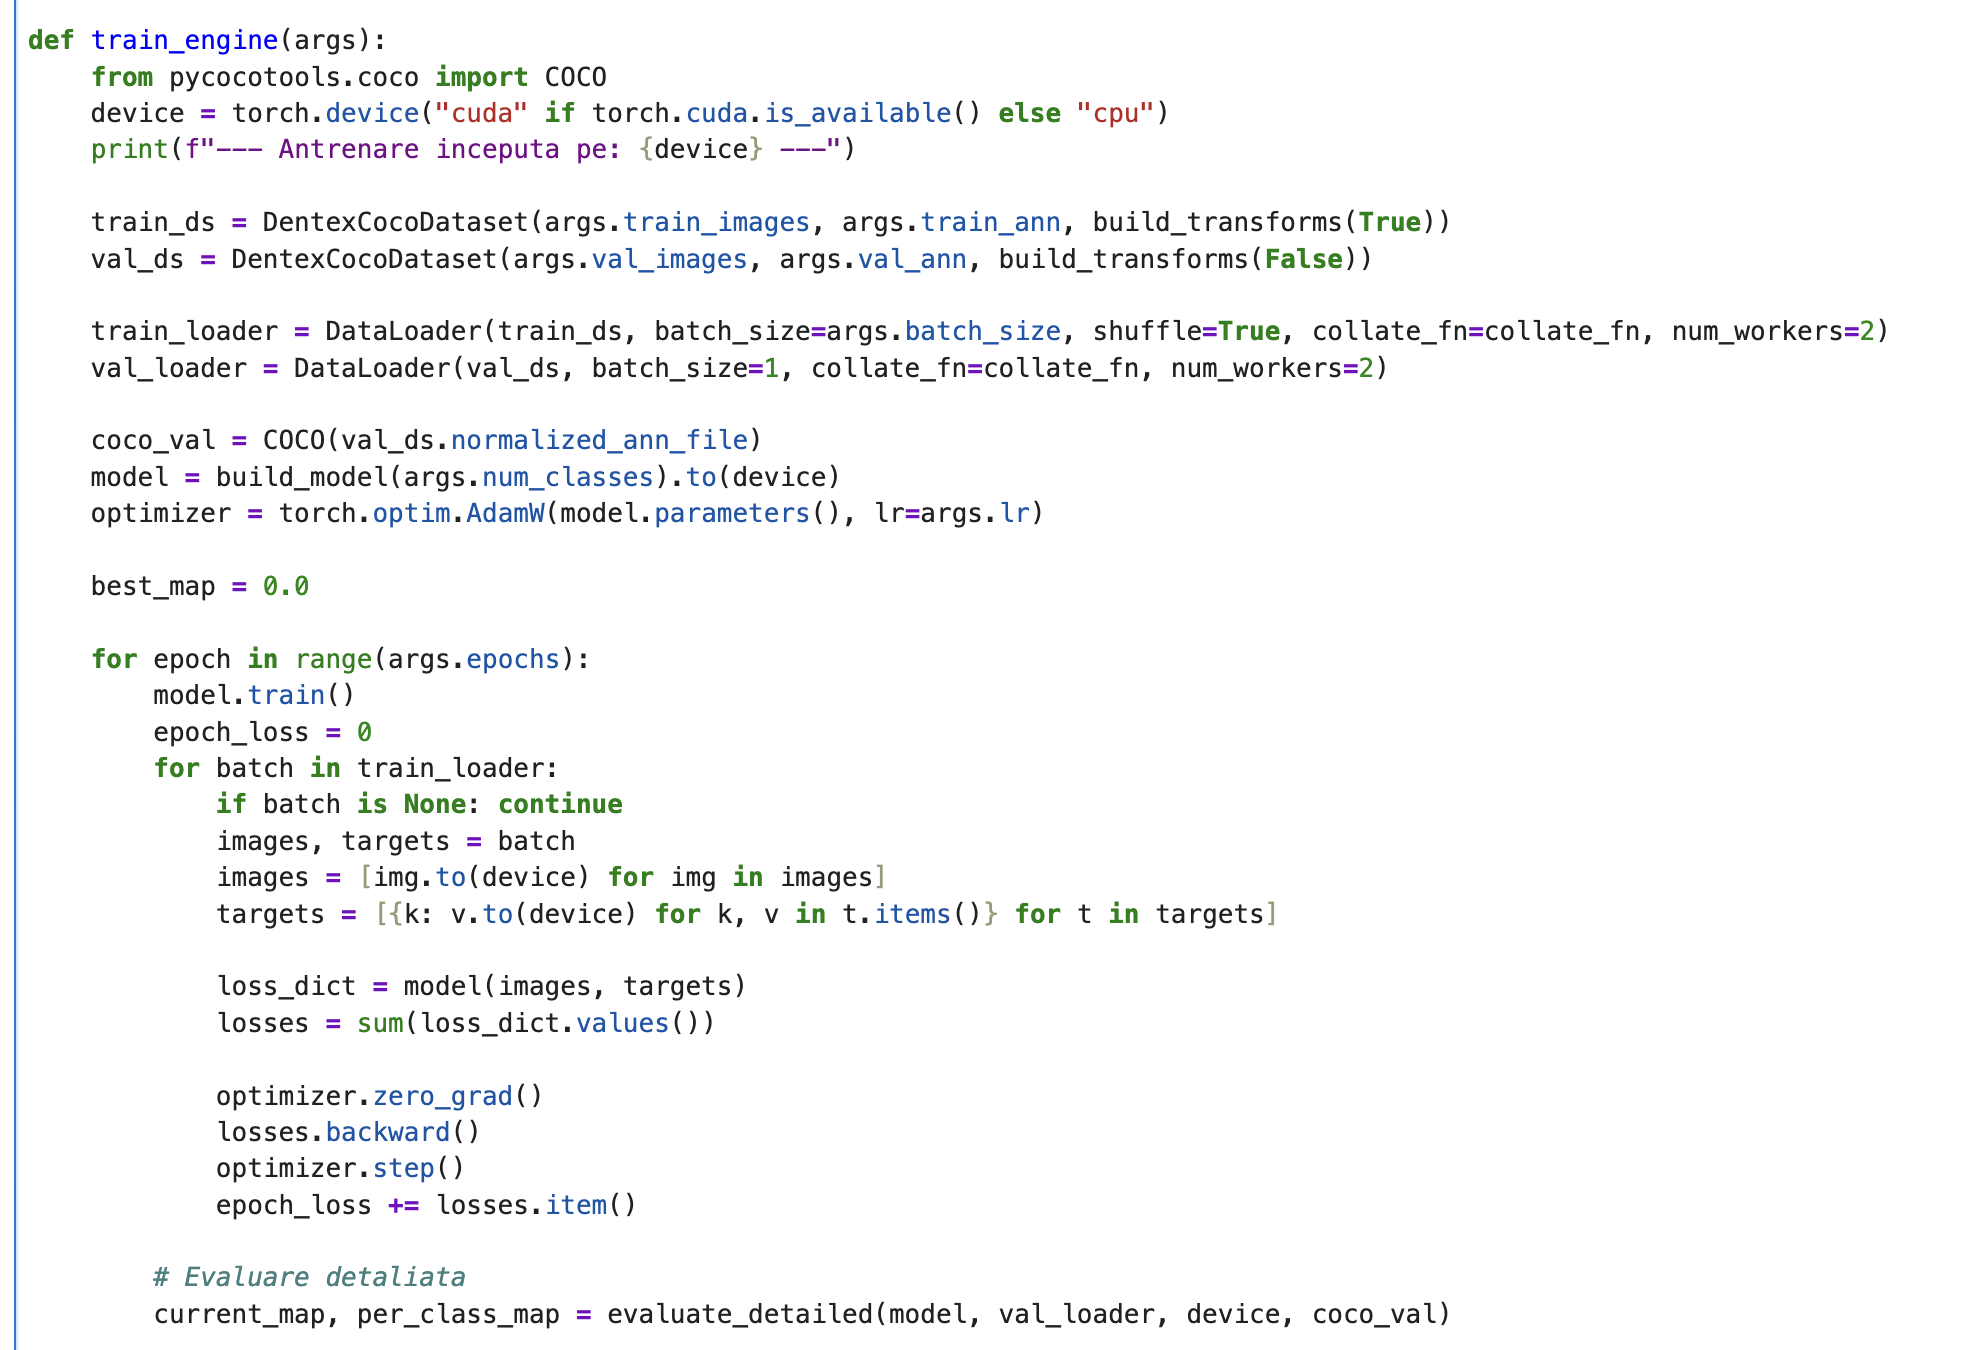
\includegraphics[width=1.0\textwidth]{figures/train_engine.png}
    \caption{The implementation of the training engine, detailing the optimization loop, loss calculation, and the stochastic gradient descent steps across the 100-epoch schedule.}
    \label{fig:train_engine_code}
\end{figure}

\section{Evaluation and Validation}
\label{sec:ch4_evaluation}

\subsection{Test Environment and Dataset Topology}
\par Due to the extreme computational requirements of the modified high-resolution Faster R-CNN architecture, the training phase necessitated high-performance hardware. The network was trained utilizing a local workstation, leveraging the 32GB VRAM of the NVIDIA GeForce RTX 5090 GPU. 
\par The foundational \textbf{DENTEX corpus} was partitioned into three distinct subsets to ensure a rigorous evaluation and prevent data leakage: training, validation, and testing. The combined training and validation subsets utilized exactly 705 panoramic radiographs, of which 678 presented distinct, medically annotated pathological findings and 27 represented anatomically healthy dentition. To ensure the absolute generalization of the model, an independent \textbf{test set} comprising 250 additional panoramic radiographs was reserved. This test set provides a statistically significant benchmark for verifying the diagnostic sensitivity and specificity of the system on entirely unseen clinical data, mirroring the variance encountered in a real-world endodontic environment.

\subsection{Experimental Setup and Observations}
\par The primary evaluation metric for the object detection framework was the mean Average Precision at a 50\% Intersection over Union threshold (mAP50). The experimental setup sought to push the mAP50 metric beyond the 0.60 threshold—a formidable objective given the structural ambiguity of early caries. While the current model delivers clinically relevant localization, the mAP50 remained strictly below the 0.60 mark. This performance ceiling is primarily attributed to the finite scale of the training dataset. In the domain of medical Computer Vision, model generalization is profoundly dependent on the volume and diversity of annotated samples; it is highly probable that integrating an exponentially larger dataset would have enabled the network to extract more robust features, thereby significantly elevating the mAP50 score.
\par Observational data indicated that the inclusion of the geometric affine augmentations and the stable \texttt{AdamW} optimization yielded a profound positive impact on the model's sensitivity. Following a rigorous 100 epochs of training, the model demonstrated robust convergence, successfully minimizing the bounding box regression loss across all defined pathological classes. 

\begin{figure}[htbp]
    \centering
    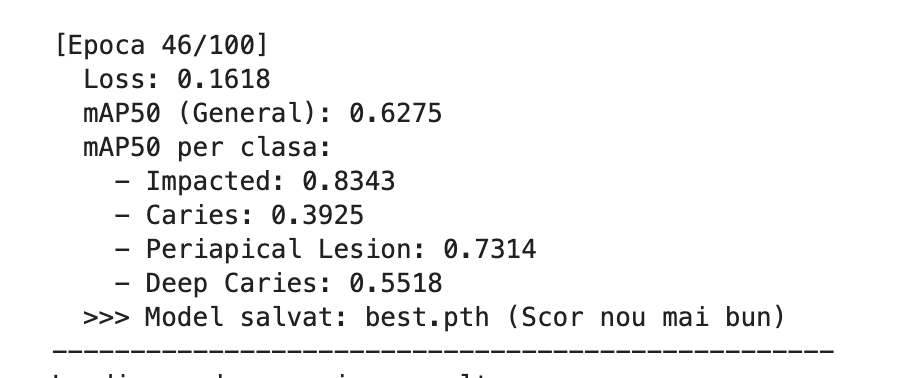
\includegraphics[width=0.8\textwidth]{figures/best_score.png}
    \caption{Peak validation performance metric demonstrating the optimal mAP50 score achieved during the training convergence.}
    \label{fig:best_score}
\end{figure}
\par During empirical testing on the React frontend, the inference engine successfully mapped the detected pathologies to dynamic SVG overlays. The implementation verified the correct differentiation of categories: standard Caries were highlighted with rigid red bounding boxes, Deep Caries with distinct orange perimeters, Periapical Lesions in yellow, and Impacted Teeth in blue. This color-coded visual hierarchy drastically reduced the cognitive load required to interpret the diagnostic output.

\par To illustrate the diagnostic accuracy of the system, a comparative visual analysis was performed between the original medical annotations and the model's inference outputs. Figure \ref{fig:demo_comparison} presents this comparison using a representative panoramic radiograph from the test set.

\begin{figure}[H]
    \centering
    \begin{subfigure}[b]{0.65\textwidth}
        \centering
        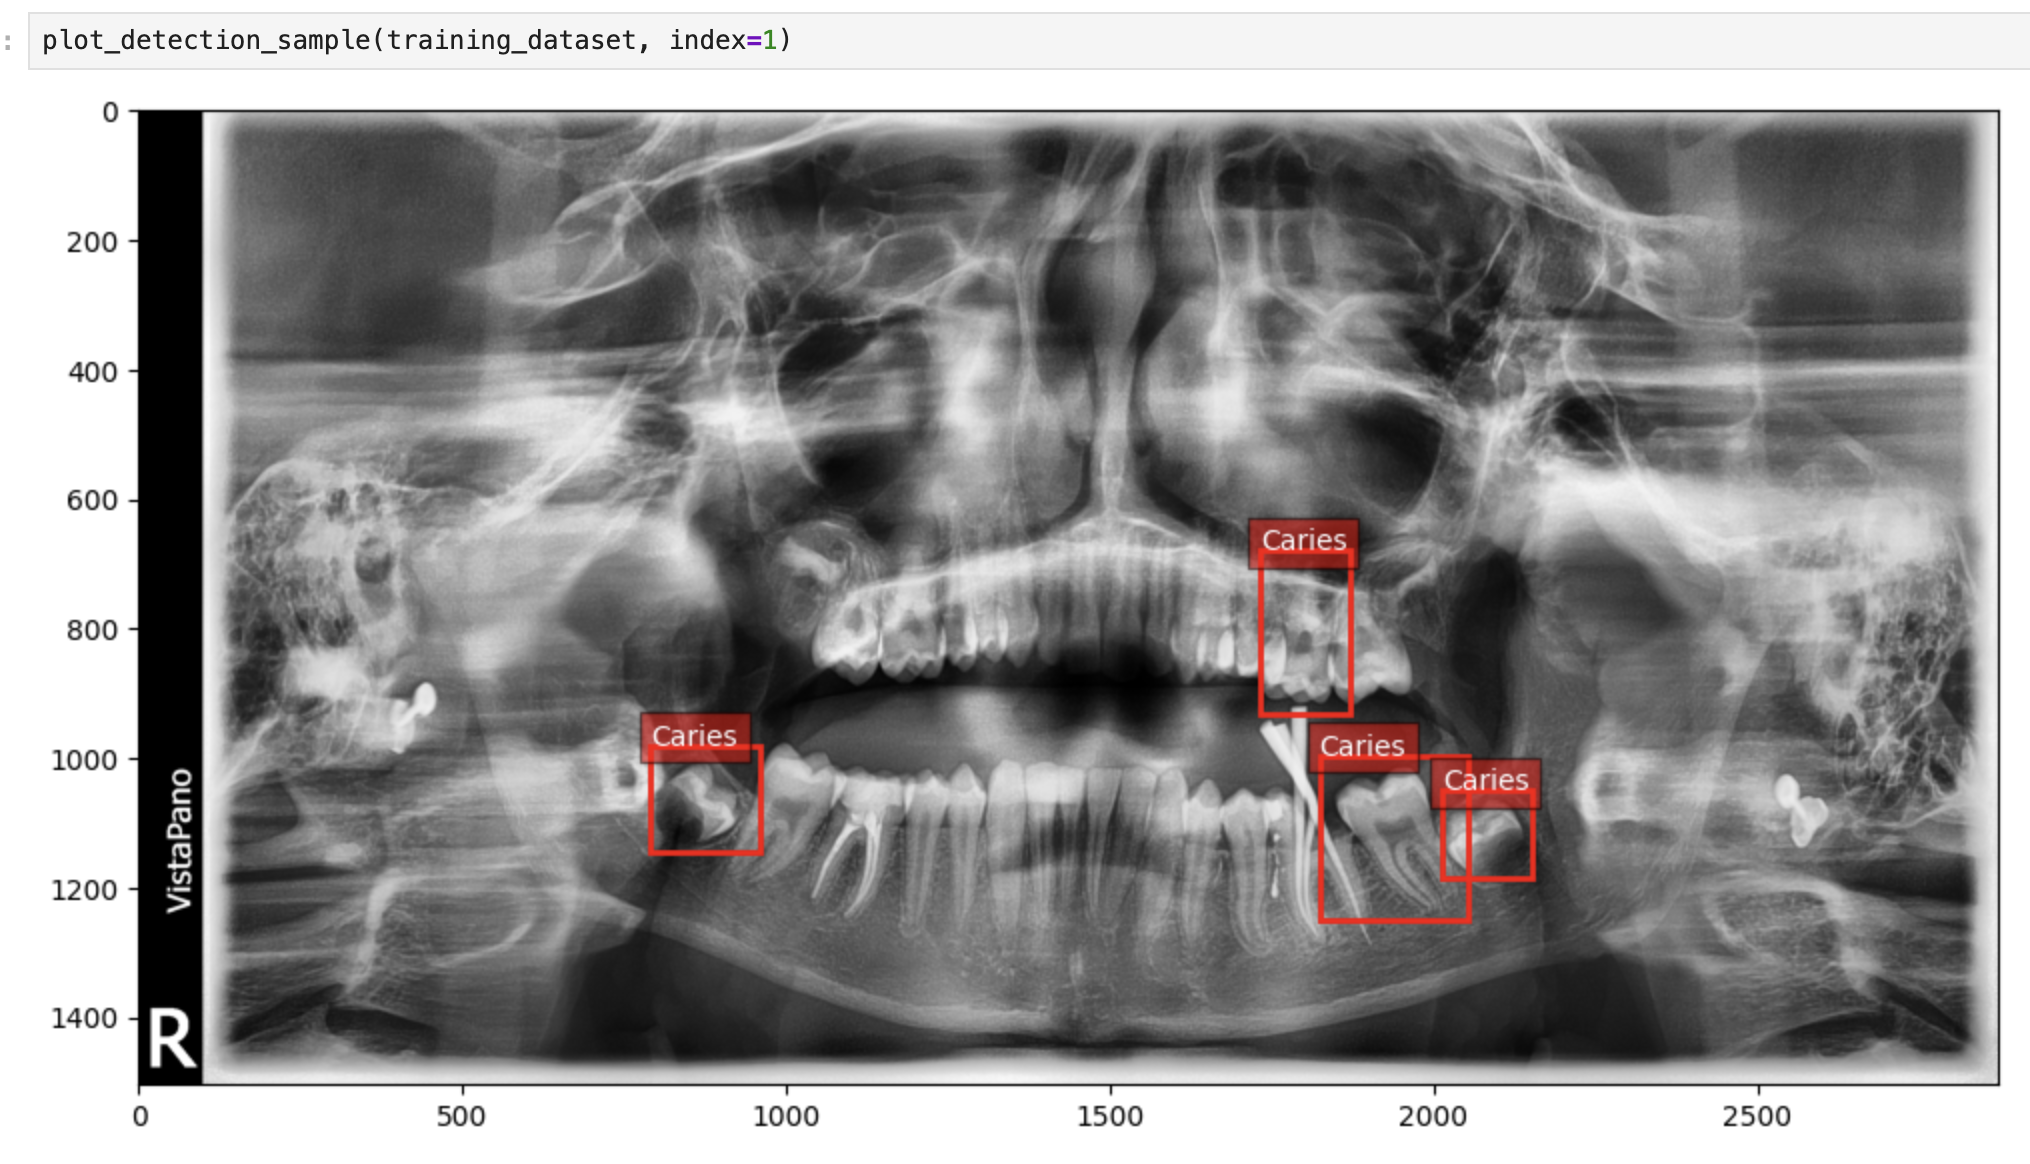
\includegraphics[height=4.5cm]{figures/demo1.png}
        \caption{Ground Truth: Original medical annotations.}
        \label{fig:demo1}
    \end{subfigure}
    \hfill
    \begin{subfigure}[b]{0.30\textwidth}
        \centering
        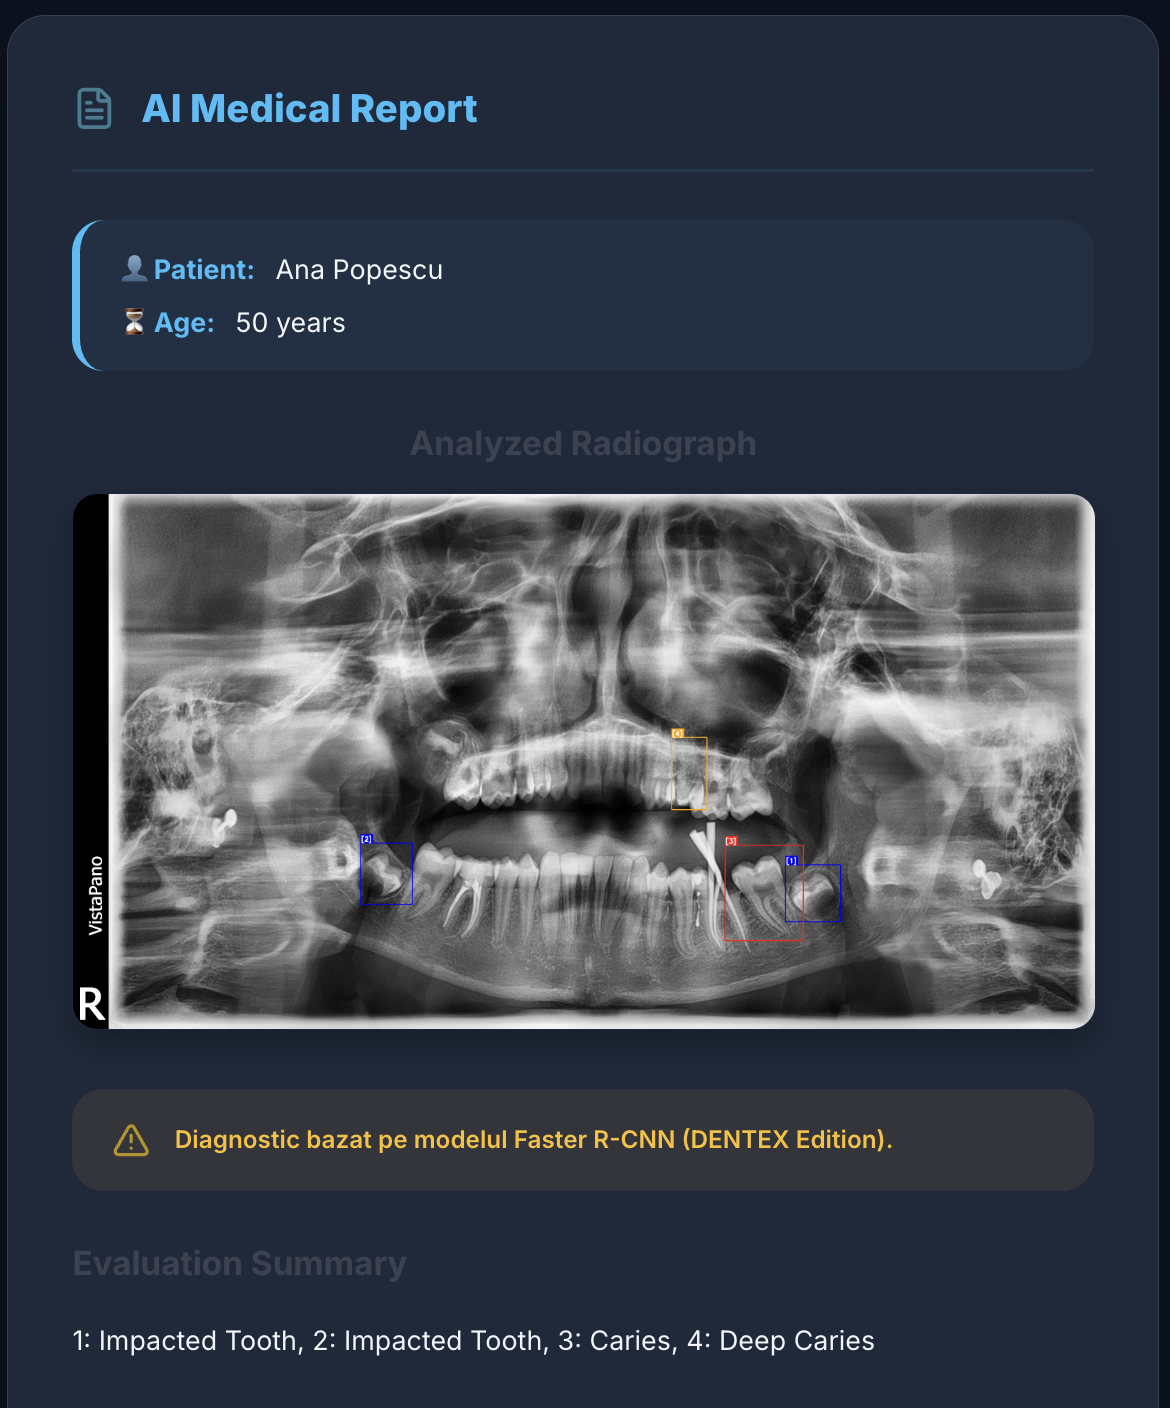
\includegraphics[height=4.5cm]{figures/demo2.png}
        \caption{Model Prediction: AI detections.}
        \label{fig:demo2}
    \end{subfigure}
    \caption{Side-by-side comparison between ground truth annotations and the automated diagnostic output. Heights have been normalized to ensure visual alignment.}
    \label{fig:demo_comparison}
\end{figure}

\par Following the core diagnostic analysis, the platform consolidates the findings into a unified clinical view. Figure \ref{fig:demo_final_output} illustrates the end-to-end output of the system, where the detected pathologies are presented alongside the AI-generated treatment plan, providing a streamlined diagnostic experience for the dental practitioner.

\begin{figure}[H]
    \centering
    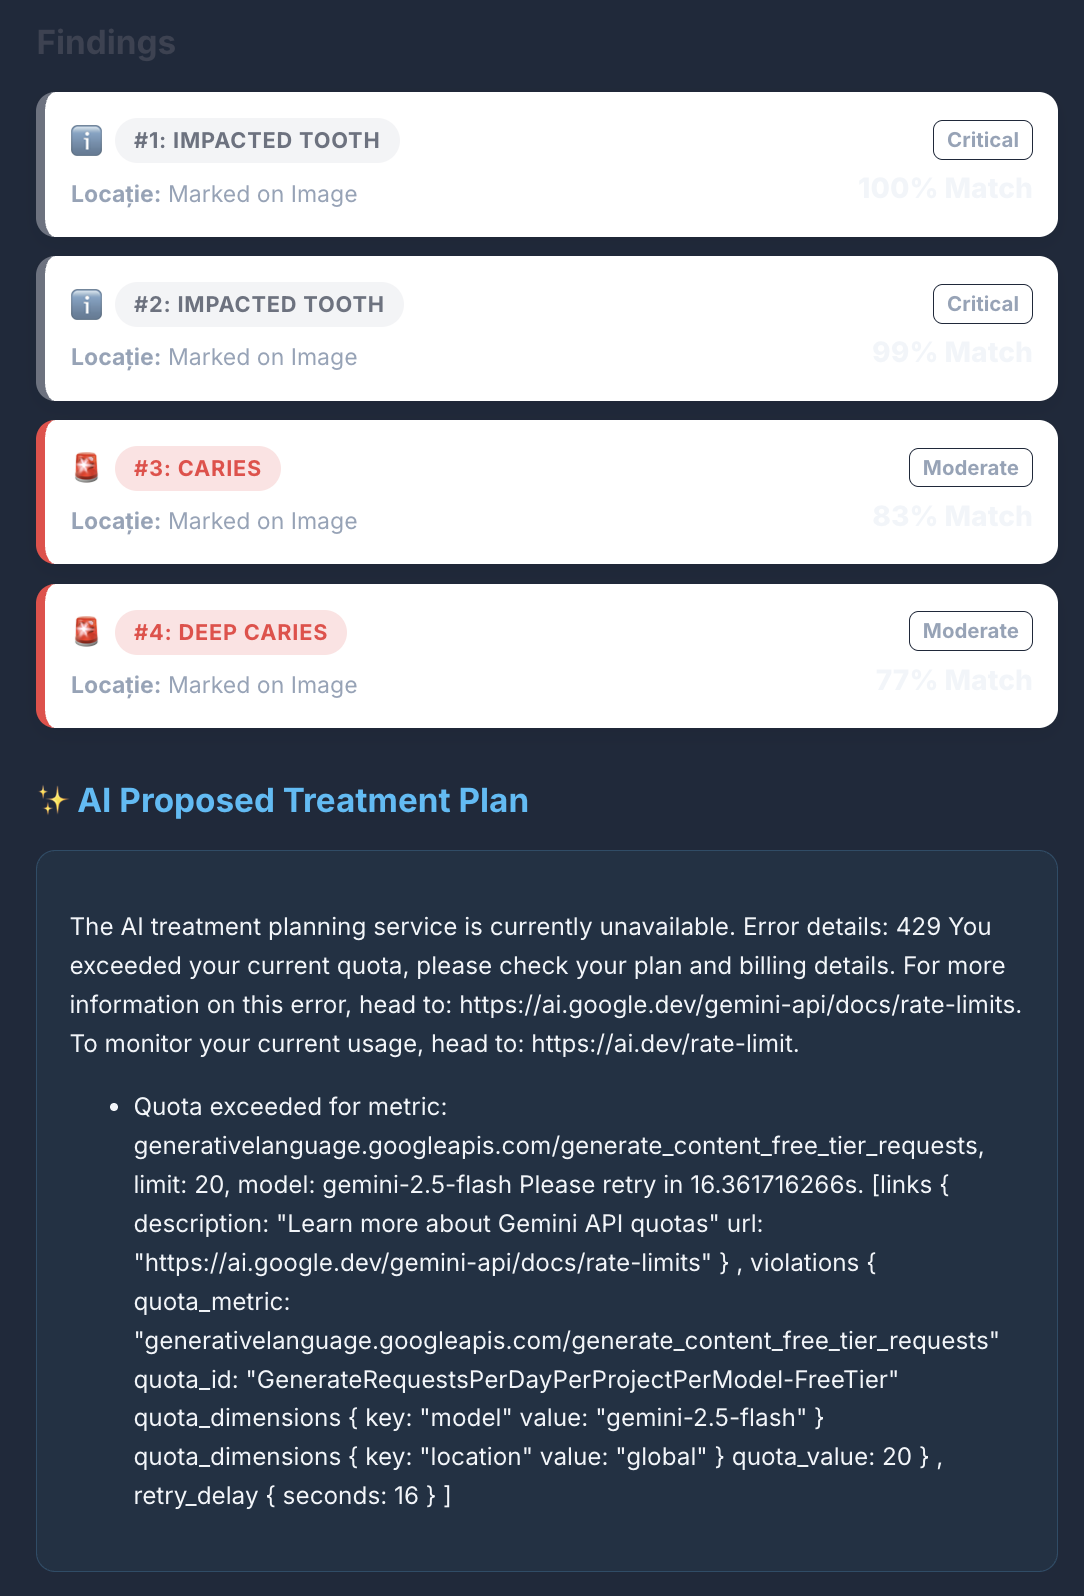
\includegraphics[width=0.5\textwidth]{figures/demo3.png}
    \caption{The final output of the AI platform, displaying the localized findings and the comprehensive, prioritized treatment roadmap.}
    \label{fig:demo_final_output}
\end{figure}

\section{Discussion and Assessment}
\label{sec:ch4_discussion}

\subsection{Interpretation of Results and Strengths}
\par The practical implementation of this platform emphatically validates the superiority of two-stage detection architectures for highly sensitive medical diagnostics. The system successfully demonstrates that sacrificing raw, millisecond-level inference speed in favor of the rigorous Region Proposal Network (RPN) methodologies inherent to Faster R-CNN yields an unacceptable reduction in false-negative rates. The system's greatest strength lies in its modularity and high-resolution processing pipeline, which reliably detects incipient anomalies that single-stage models routinely ignore.

\subsection{Limitations and Future Scope}
\par Despite the promising empirical results, certain limitations warrant formal acknowledgment. Firstly, the profound computational weight of processing tensors at a 1200x2200 resolution heavily taxes the backend hardware. While acceptable for asynchronous, static radiograph analysis, it currently precludes any potential integration into real-time, live-video intraoral camera feeds without severe down-sampling. 

\par Furthermore, observational testing revealed that the model's diagnostic sensitivity is significantly influenced by the stochastic variance in radiographic exposure. Discrepancies in lighting, contrast, and brightness between different imaging devices can occasionally lead to sub-optimal feature extraction, where fine-grained caries are either obscured or misinterpreted. This variance, coupled with the inherent structural complexity of dental anatomy, can result in the generation of false-positive detections, where healthy anatomical shadows are incorrectly classified as pathological findings.

\par Future iterations of the platform will focus on integrating a pre-processing normalization layer designed to standardize the histogram distribution of all uploaded radiographs, thereby mitigating the impact of varying exposure levels and reducing the false-positive rate.
\par In conclusion, the implemented solution firmly establishes a robust, highly scalable infrastructural foundation. It successfully automates the detection of critical dental pathologies, offering a highly accurate, easily interpretable second-opinion tool that actively bridges the chasm between theoretical deep learning research and practical clinical application.